\documentclass{standalone}
\usepackage{tikz}
\usetikzlibrary{shapes.geometric, positioning} % Added positioning library for 'below of' option

\begin{document}
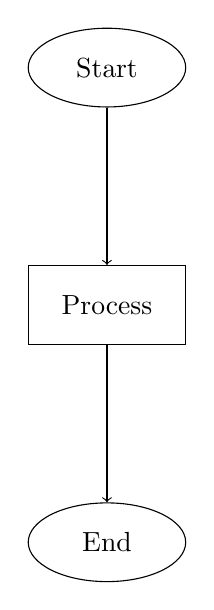
\begin{tikzpicture}[node distance=2cm]
  % Define node styles using \tikzset instead of deprecated \tikzstyle
  \tikzset{
    start/.style={ellipse, draw, minimum width=2cm, minimum height=1cm},
    process/.style={rectangle, draw, minimum width=2cm, minimum height=1cm},
    end/.style={ellipse, draw, minimum width=2cm, minimum height=1cm}
  }

  % Create nodes
  \node (start) [start] {Start};
  \node (process) [process, below=of start] {Process}; % Changed 'below of' to 'below'
  \node (end) [end, below=of process] {End}; % Changed 'below of' to 'below'

  % Draw arrows between nodes
  \draw[->] (start) -- (process);
  \draw[->] (process) -- (end);

\end{tikzpicture}
\end{document}